\section{Validation Strategies}
\begin{frame}{Detecting Overfitting: The Holdout Split}
    \begin{itemize}
        \item We cannot trust performance on training data (memorization).
        \item \textbf{Solution:} Hide a piece of data to simulate the "Future."
    \end{itemize}
    
    \vspace{1em} % Increased vertical space before diagram
    \centering
    
    % Adjusted scale and width (0 to 12 instead of 0 to 10)
    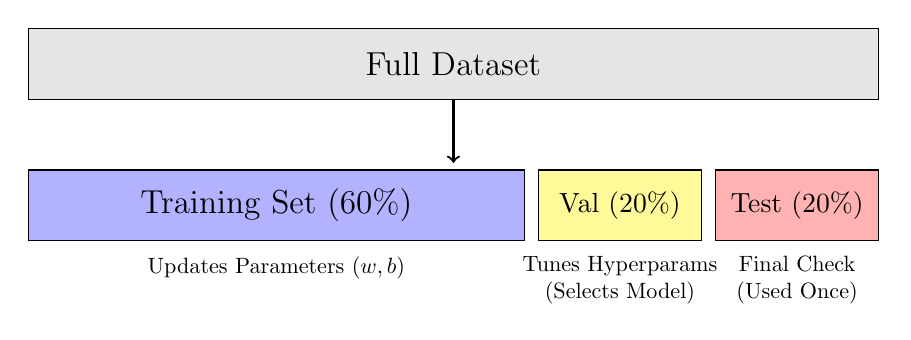
\begin{tikzpicture}[scale=0.9]
    
         % --- Full Data (Top) ---
         % Stretched width to 12, moved up to y=1.5
         \draw[fill=gray!20] (0,1.5) rectangle (12,2.5);
         \node at (6,2.0) {\large Full Dataset};
         
         % Arrow (Longer now)
         \draw[->, thick] (6,1.5) -- (6,0.6);
         
         % --- Splits (Bottom) ---
         
         % 1. Training Set (Widen to 7 units)
         \draw[fill=blue!30] (0,-0.5) rectangle (7,0.5);
         \node at (3.5,0) {\large Training Set (60\%)};
         % Text below with fixed width for cleaner wrapping
         \node[below=1mm, align=center, text width=6cm, scale=0.8] at (3.5,-0.5) 
              {Updates Parameters ($w, b$)};
         
         % 2. Validation Set (Widen to 2.3 units)
         \draw[fill=yellow!40] (7.2,-0.5) rectangle (9.5,0.5);
         \node at (8.35,0) {Val (20\%)};
         \node[below=1mm, align=center, text width=3.5cm, scale=0.8] at (8.35,-0.5) 
              {Tunes Hyperparams\\(Selects Model)};
         
         % 3. Test Set (Widen to 2.3 units)
         \draw[fill=red!30] (9.7,-0.5) rectangle (12,0.5);
         \node at (10.85,0) {Test (20\%)};
         \node[below=1mm, align=center, text width=2.5cm, scale=0.8] at (10.85,-0.5) 
              {Final Check\\(Used Once)};
              
    \end{tikzpicture}
\end{frame}

\begin{frame}{Diagnosis: Loss Curves}
    \vspace{0.5em}
    \centering
    \begin{columns}[T]
        % Column 1: Underfit
        \begin{column}{0.32\textwidth}
            \centering
            \colorbox{gray!10}{\parbox{1.05\textwidth}{
                \centering
                \vspace{0.3em}
                \textbf{\large Underfitting}\\[0.4em]
                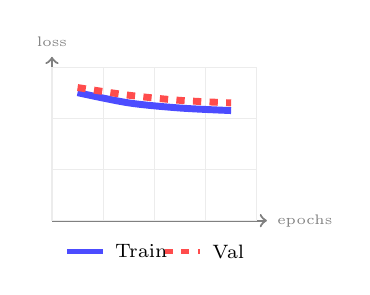
\begin{tikzpicture}[scale=0.65]
                    \draw[->, thick, gray] (0,0) -- (4.2,0) node[right, font=\tiny] {epochs};
                    \draw[->, thick, gray] (0,0) -- (0,3.2) node[above, font=\tiny] {loss};
                    \draw[gray!15, thin] (0,0) grid (4,3);
                    
                    % Train
                    \draw[blue!70, line width=2.5pt] plot[smooth] coordinates {(0.5,2.5) (1.5,2.3) (2.5,2.2) (3.5,2.15)};
                    % Val
                    \draw[red!70, line width=2.5pt, dashed] plot[smooth] coordinates {(0.5,2.6) (1.5,2.45) (2.5,2.35) (3.5,2.3)};
                    
                    % Legend
                    \draw[blue!70, line width=2pt] (0.3,-0.6) -- (1,-0.6) node[right, font=\scriptsize, black] {Train};
                    \draw[red!70, line width=2pt, dashed] (2.2,-0.6) -- (2.9,-0.6) node[right, font=\scriptsize, black] {Val};
                \end{tikzpicture}\\[0.5em]
                {\small Both losses remain \textbf{high}}\\
                {\scriptsize\color{gray} Model too simple}\\[0.3em]
            }}
        \end{column}
        
        % Column 2: Good Fit
        \begin{column}{0.32\textwidth}
            \centering
            \colorbox{green!8}{\parbox{1.05\textwidth}{
                \centering
                \vspace{0.3em}
                \textbf{\large Good Fit}\\[0.4em]
                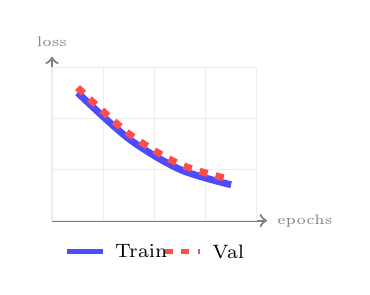
\begin{tikzpicture}[scale=0.65]
                    \draw[->, thick, gray] (0,0) -- (4.2,0) node[right, font=\tiny] {epochs};
                    \draw[->, thick, gray] (0,0) -- (0,3.2) node[above, font=\tiny] {loss};
                    \draw[gray!15, thin] (0,0) grid (4,3);
                    
                    % Train
                    \draw[blue!70, line width=2.5pt] plot[smooth] coordinates {(0.5,2.5) (1.5,1.6) (2.5,1.0) (3.5,0.7)};
                    % Val
                    \draw[red!70, line width=2.5pt, dashed] plot[smooth] coordinates {(0.5,2.6) (1.5,1.7) (2.5,1.1) (3.5,0.8)};
                    
                    % Legend
                    \draw[blue!70, line width=2pt] (0.3,-0.6) -- (1,-0.6) node[right, font=\scriptsize, black] {Train};
                    \draw[red!70, line width=2pt, dashed] (2.2,-0.6) -- (2.9,-0.6) node[right, font=\scriptsize, black] {Val};
                \end{tikzpicture}\\[0.5em]
                {\small Both losses are \textbf{low}}\\
                {\scriptsize\color{gray} Curves track down closely}\\[0.3em]
            }}
        \end{column}
        
        % Column 3: Overfit
        \begin{column}{0.32\textwidth}
            \centering
            \colorbox{orange!10}{\parbox{1.05\textwidth}{
                \centering
                \vspace{0.3em}
                \textbf{\large Overfitting}\\[0.4em]
                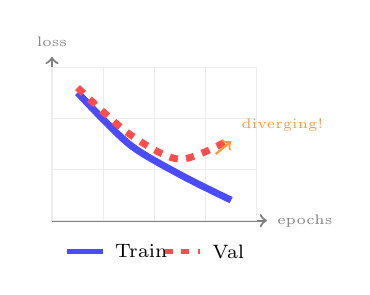
\begin{tikzpicture}[scale=0.65]
                    \draw[->, thick, gray] (0,0) -- (4.2,0) node[right, font=\tiny] {epochs};
                    \draw[->, thick, gray] (0,0) -- (0,3.2) node[above, font=\tiny] {loss};
                    \draw[gray!15, thin] (0,0) grid (4,3);
                    
                    % Train
                    \draw[blue!70, line width=2.5pt] plot[smooth] coordinates {(0.5,2.5) (1.5,1.5) (2.5,0.9) (3.5,0.4)};
                    % Val
                    \draw[red!70, line width=2.5pt, dashed] plot[smooth] coordinates {(0.5,2.6) (1.5,1.7) (2.5,1.2) (3.5,1.6)};
                    
                    % Annotation arrow
                    \draw[->, orange!80, thick] (3.2,1.3) -- (3.5,1.55) node[above right, font=\tiny] {diverging!};
                    
                    % Legend
                    \draw[blue!70, line width=2pt] (0.3,-0.6) -- (1,-0.6) node[right, font=\scriptsize, black] {Train};
                    \draw[red!70, line width=2pt, dashed] (2.2,-0.6) -- (2.9,-0.6) node[right, font=\scriptsize, black] {Val};
                \end{tikzpicture}\\[0.5em]
                {\small Train loss ↓, Val loss ↑}\\
                {\scriptsize\color{gray} Model started to overfit!}\\[0.3em]
            }}
        \end{column}
    \end{columns}
    
    \vspace{1em}
    \begin{center}
        \small\textit{The gap between training and validation loss reveals overfitting!}
    \end{center}
\end{frame}

\begin{frame}{Detecting Overfitting: The Holdout Split}
    
    \centering
    
    % Adjusted scale and width (0 to 12 instead of 0 to 10)
    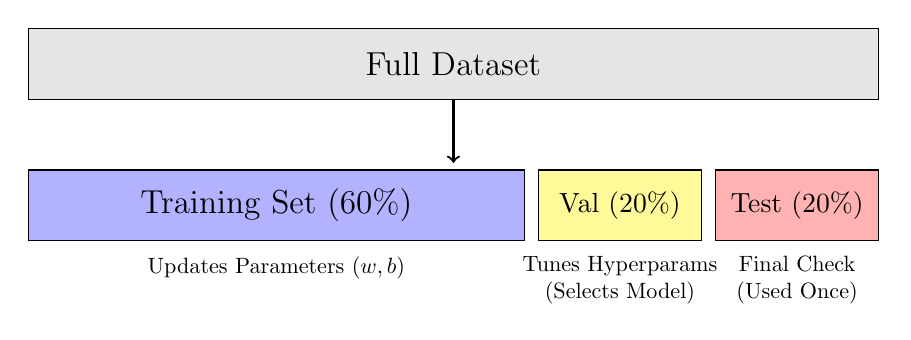
\begin{tikzpicture}[scale=0.9]
    
         % --- Full Data (Top) ---
         % Stretched width to 12, moved up to y=1.5
         \draw[fill=gray!20] (0,1.5) rectangle (12,2.5);
         \node at (6,2.0) {\large Full Dataset};
         
         % Arrow (Longer now)
         \draw[->, thick] (6,1.5) -- (6,0.6);
         
         % --- Splits (Bottom) ---
         
         % 1. Training Set (Widen to 7 units)
         \draw[fill=blue!30] (0,-0.5) rectangle (7,0.5);
         \node at (3.5,0) {\large Training Set (60\%)};
         % Text below with fixed width for cleaner wrapping
         \node[below=1mm, align=center, text width=6cm, scale=0.8] at (3.5,-0.5) 
              {Updates Parameters ($w, b$)};
         
         % 2. Validation Set (Widen to 2.3 units)
         \draw[fill=yellow!40] (7.2,-0.5) rectangle (9.5,0.5);
         \node at (8.35,0) {Val (20\%)};
         \node[below=1mm, align=center, text width=3.5cm, scale=0.8] at (8.35,-0.5) 
              {Tunes Hyperparams\\(Selects Model)};
         
         % 3. Test Set (Widen to 2.3 units)
         \draw[fill=red!30] (9.7,-0.5) rectangle (12,0.5);
         \node at (10.85,0) {Test (20\%)};
         \node[below=1mm, align=center, text width=2.5cm, scale=0.8] at (10.85,-0.5) 
              {Final Check\\(Used Once)};
              
              
    \end{tikzpicture}

    \begin{itemize}
        \item While this split works conceptually, we may encounter several problems in practice... 
    \end{itemize}
\end{frame}

% --- SLIDE 1: The Problem (Ordered Data) ---
\begin{frame}{The Problem: Ordered Data}
    
    \begin{columns}[c]
        % --- Left Column: The Logic ---
        \begin{column}{0.45\textwidth}
            \textbf{Data is Often Ordered}
            \begin{itemize}
                \item Real-world data is often collected sequentially (by date, time, or class).
                \item If we split data directly, the model trains on one pattern but gets tested on a completely different one.
            \end{itemize}
        \end{column}
        
        % --- Right Column: The Visuals ---
        \begin{column}{0.55\textwidth}
            \centering
            
            \textbf{1. Ordered Split (Biased)}
            \vspace{0.2em}
            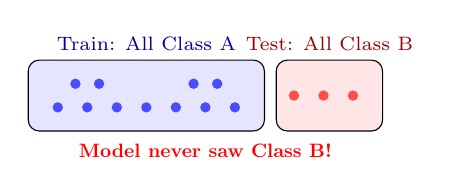
\begin{tikzpicture}[scale=0.75]
                % Train Box (Blue Region)
                \draw[fill=blue!10, rounded corners] (0,0) rectangle (4,1.2);
                \node[above, font=\scriptsize, blue!60!black] at (2,1.2) {Train: All Class A};
                \foreach \x in {0.5,1,1.5,2,2.5,3,3.5} \fill[blue!70] (\x, 0.4) circle (2.5pt);
                \foreach \x in {0.8,1.2,2.8,3.2} \fill[blue!70] (\x, 0.8) circle (2.5pt);
                
                % Test Box (Red Region)
                \draw[fill=red!10, rounded corners] (4.2,0) rectangle (6,1.2);
                \node[above, font=\scriptsize, red!60!black] at (5.1,1.2) {Test: All Class B};
                \foreach \x in {4.5,5,5.5} \fill[red!70] (\x, 0.6) circle (2.5pt);
                
                % Warning
                \node[below, red, font=\bfseries, scale=0.7] at (3, -0.1) {Model never saw Class B!};
            \end{tikzpicture}
            
            \vspace{1em}
            
            
        \end{column}
    \end{columns}

    
    
\end{frame}


% --- SLIDE 1: The Problem (Ordered Data) ---
\begin{frame}{The Problem: Ordered Data}
    
    \begin{columns}[c]
        % --- Left Column: The Logic ---
        \begin{column}{0.45\textwidth}
            \textbf{Data is Often Ordered}
            \begin{itemize}
                \item Real-world data is often collected sequentially (by date, time, or class).
                \item If we split data directly, the model trains on one pattern but gets tested on a completely different one.
            \end{itemize}
            
            \vspace{1em}
            \begin{block}{Solution: }Shuffle the data before splitting!
            \end{block}
        \end{column}
        
        % --- Right Column: The Visuals ---
        \begin{column}{0.55\textwidth}
            \centering
            
            \textbf{1. Ordered Split (Biased)}
            \vspace{0.2em}
            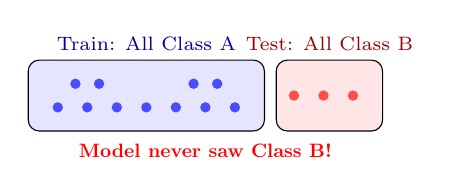
\begin{tikzpicture}[scale=0.75]
                % Train Box (Blue Region)
                \draw[fill=blue!10, rounded corners] (0,0) rectangle (4,1.2);
                \node[above, font=\scriptsize, blue!60!black] at (2,1.2) {Train: All Class A};
                \foreach \x in {0.5,1,1.5,2,2.5,3,3.5} \fill[blue!70] (\x, 0.4) circle (2.5pt);
                \foreach \x in {0.8,1.2,2.8,3.2} \fill[blue!70] (\x, 0.8) circle (2.5pt);
                
                % Test Box (Red Region)
                \draw[fill=red!10, rounded corners] (4.2,0) rectangle (6,1.2);
                \node[above, font=\scriptsize, red!60!black] at (5.1,1.2) {Test: All Class B};
                \foreach \x in {4.5,5,5.5} \fill[red!70] (\x, 0.6) circle (2.5pt);
                
                % Warning
                \node[below, red, font=\bfseries, scale=0.7] at (3, -0.1) {Model never saw Class B!};
            \end{tikzpicture}
            
            \vspace{1em}
            
            \textbf{2. Shuffled Split (Correct)}
            \vspace{0.2em}
            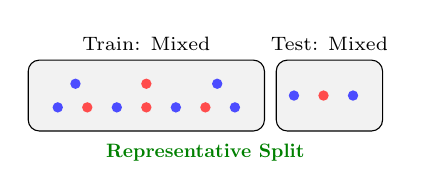
\begin{tikzpicture}[scale=0.75]
                % Train Box (Mixed)
                \draw[fill=gray!10, rounded corners] (0,0) rectangle (4,1.2);
                \node[above, font=\scriptsize] at (2,1.2) {Train: Mixed};
                % Mix of Blue and Red
                \foreach \x in {0.5,1.5,2.5,3.5} \fill[blue!70] (\x, 0.4) circle (2.5pt);
                \foreach \x in {1.0,2.0,3.0} \fill[red!70] (\x, 0.4) circle (2.5pt);
                \foreach \x in {0.8,3.2} \fill[blue!70] (\x, 0.8) circle (2.5pt);
                \foreach \x in {2.0} \fill[red!70] (\x, 0.8) circle (2.5pt);
                
                % Test Box (Mixed)
                \draw[fill=gray!10, rounded corners] (4.2,0) rectangle (6,1.2);
                \node[above, font=\scriptsize] at (5.1,1.2) {Test: Mixed};
                \fill[blue!70] (4.5, 0.6) circle (2.5pt);
                \fill[red!70] (5.0, 0.6) circle (2.5pt);
                \fill[blue!70] (5.5, 0.6) circle (2.5pt);
                
                % Success
                \node[below, green!50!black, font=\bfseries, scale=0.7] at (3, -0.1) { Representative Split \checkmark};
            \end{tikzpicture}
        \end{column}
    \end{columns}

    
    
\end{frame}

% --- SLIDE 1: The Problem (Ordered Data) ---
\begin{frame}{The Problem: Ordered Data}
    
    \begin{columns}[c]
        % --- Left Column: The Logic ---
        \begin{column}{0.45\textwidth}
            \textbf{Data is Often Ordered}
            \begin{itemize}
                \item Real-world data is often collected sequentially (by date, time, or class).
                \item If we split data directly, the model trains on one pattern but gets tested on a completely different one.
            \end{itemize}
            
            \vspace{1em}
            \begin{block}{Solution: }Shuffle the data before splitting!
            \end{block}
            \vspace{1em}
            \begin{block}{This helps, but what if data is small?}
            \end{block}
        \end{column}
        
        % --- Right Column: The Visuals ---
        \begin{column}{0.55\textwidth}
            \centering
            
            \textbf{1. Ordered Split (Biased)}
            \vspace{0.2em}
            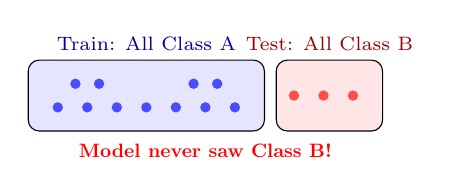
\begin{tikzpicture}[scale=0.75]
                % Train Box (Blue Region)
                \draw[fill=blue!10, rounded corners] (0,0) rectangle (4,1.2);
                \node[above, font=\scriptsize, blue!60!black] at (2,1.2) {Train: All Class A};
                \foreach \x in {0.5,1,1.5,2,2.5,3,3.5} \fill[blue!70] (\x, 0.4) circle (2.5pt);
                \foreach \x in {0.8,1.2,2.8,3.2} \fill[blue!70] (\x, 0.8) circle (2.5pt);
                
                % Test Box (Red Region)
                \draw[fill=red!10, rounded corners] (4.2,0) rectangle (6,1.2);
                \node[above, font=\scriptsize, red!60!black] at (5.1,1.2) {Test: All Class B};
                \foreach \x in {4.5,5,5.5} \fill[red!70] (\x, 0.6) circle (2.5pt);
                
                % Warning
                \node[below, red, font=\bfseries, scale=0.7] at (3, -0.1) {Model never saw Class B!};
            \end{tikzpicture}
            
            \vspace{1em}
            
            \textbf{2. Shuffled Split (Correct)}
            \vspace{0.2em}
            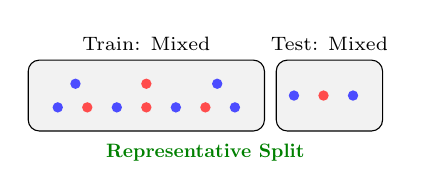
\begin{tikzpicture}[scale=0.75]
                % Train Box (Mixed)
                \draw[fill=gray!10, rounded corners] (0,0) rectangle (4,1.2);
                \node[above, font=\scriptsize] at (2,1.2) {Train: Mixed};
                % Mix of Blue and Red
                \foreach \x in {0.5,1.5,2.5,3.5} \fill[blue!70] (\x, 0.4) circle (2.5pt);
                \foreach \x in {1.0,2.0,3.0} \fill[red!70] (\x, 0.4) circle (2.5pt);
                \foreach \x in {0.8,3.2} \fill[blue!70] (\x, 0.8) circle (2.5pt);
                \foreach \x in {2.0} \fill[red!70] (\x, 0.8) circle (2.5pt);
                
                % Test Box (Mixed)
                \draw[fill=gray!10, rounded corners] (4.2,0) rectangle (6,1.2);
                \node[above, font=\scriptsize] at (5.1,1.2) {Test: Mixed};
                \fill[blue!70] (4.5, 0.6) circle (2.5pt);
                \fill[red!70] (5.0, 0.6) circle (2.5pt);
                \fill[blue!70] (5.5, 0.6) circle (2.5pt);
                
                % Success
                \node[below, green!50!black, font=\bfseries, scale=0.7] at (3, -0.1) { Representative Split \checkmark};
            \end{tikzpicture}
        \end{column}
    \end{columns}

    
    
\end{frame}

% --- SLIDE 2: But What If Data is Small? ---
\begin{frame}{What If Data is Small?}

    \begin{block}{The Remaining Problem}
        Shuffling fixes the \textit{order} bias, but with small datasets, a single random split can still be \textbf{unlucky}.
    \end{block}

    % \vspace{0.5em}
    
    \begin{columns}[c]
        % --- Left Column: Text Explanation (Narrower) ---
        \begin{column}{0.40\textwidth}
            \textbf{The Law of Small Numbers:}
            
            \begin{itemize}
                \item 20\% of a small dataset is a tiny sample.
                \item It is statistically likely that this small sample will not match the population perfectly.
                \item \textbf{Result:} We get "Lucky" or "Unlucky" splits.
            \end{itemize}
        \end{column}
        
        % --- Right Column: The Visuals (Wider) ---
        \begin{column}{0.65\textwidth}
            \centering
            
            % LEGEND (Centered)
            
\begin{tikzpicture}[scale=0.7]
                 \fill[blue!70] (0,0) circle (3pt); 
                 \node[right, scale=0.8] at (0.1,0) {Standard};
                 
                 \node[red, font=\bfseries] at (2.5,0) {x}; 
                 \node[right, scale=0.8] at (2.7,0) {Hard Case};
            \end{tikzpicture}
            
            \vspace{0.5em}
            
            % SCENARIO A: LUCKY
            \textbf{Scenario A: "Lucky" Split}
            \vspace{0.2em}
            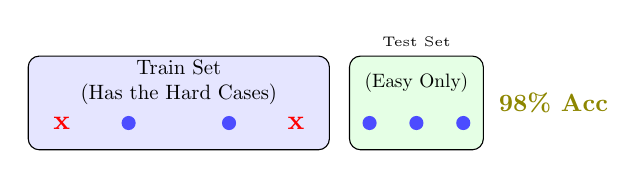
\begin{tikzpicture}[scale=0.85]
                % Train Box (Stretched width to 4.5)
                \draw[fill=blue!10, rounded corners] (0,0) rectangle (4.5,1.4);
                % Text Centered
                \node[scale=0.75, align=center] at (2.25, 1.0) {Train Set\\(Has the Hard Cases)};
                % Markers spread out
                \node[red, font=\bfseries] at (0.5,0.4) {x}; 
                \node[red, font=\bfseries] at (4.0,0.4) {x};
                \fill[blue!70] (1.5,0.4) circle (3pt);
                \fill[blue!70] (3.0,0.4) circle (3pt);
                
                % Test Box (Stretched & Shifted)
                \draw[fill=green!10, rounded corners] (4.8,0) rectangle (6.8,1.4);
                \node[above, font=\tiny] at (5.8,1.4) {Test Set};
                \node[scale=0.7, align=center] at (5.8, 1.0) {(Easy Only)};
                % Test has ONLY Blue Dots
                \fill[blue!70] (5.1, 0.4) circle (3pt); 
                \fill[blue!70] (5.8, 0.4) circle (3pt); 
                \fill[blue!70] (6.5, 0.4) circle (3pt);
                
                \node[right, olive, font=\bfseries, scale=0.9] at (6.9, 0.7) {98\% Acc};
            \end{tikzpicture}
            
            \vspace{0.8em}
            
            % SCENARIO B: UNLUCKY
            \textbf{Scenario B: "Unlucky" Split}
            \vspace{0.2em}
            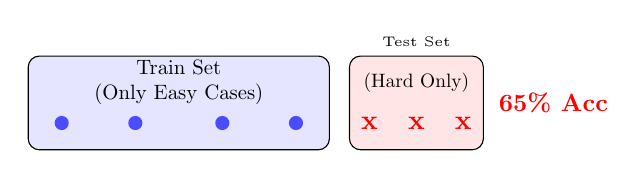
\begin{tikzpicture}[scale=0.85]
                % Train Box
                \draw[fill=blue!10, rounded corners] (0,0) rectangle (4.5,1.4);
                % Text Centered
                \node[scale=0.75, align=center] at (2.25, 1.0) {Train Set\\(Only Easy Cases)};
                % Markers spread out
                \fill[blue!70] (0.5,0.4) circle (3pt); 
                \fill[blue!70] (1.6,0.4) circle (3pt); 
                \fill[blue!70] (2.9,0.4) circle (3pt);
                \fill[blue!70] (4.0,0.4) circle (3pt);
                
                % Test Box
                \draw[fill=red!10, rounded corners] (4.8,0) rectangle (6.8,1.4);
                \node[above, font=\tiny] at (5.8,1.4) {Test Set};
                \node[scale=0.7, align=center] at (5.8, 1.0) {(Hard Only)};
                % Test has THE RED Xs
                \node[red, font=\bfseries] at (5.1, 0.4) {x}; 
                \node[red, font=\bfseries] at (5.8, 0.4) {x}; 
                \node[red, font=\bfseries] at (6.5, 0.4) {x};
                
                \node[right, red, font=\bfseries, scale=0.9] at (6.9, 0.7) {65\% Acc};
            \end{tikzpicture}
            
            \vspace{0.5em}
            {\small\textit{Same data, just a different random cut!}}
        \end{column}
    \end{columns}
\end{frame}

\definecolor{darkred}{rgb}{0.5,0,0}
\definecolor{darkblue}{RGB}{0,0,139}


% --- SLIDE 3: K-FOLD SOLUTION ---
\begin{frame}{The Solution: K-Fold Cross Validation}

    \textbf{Use ALL Data for Testing (Across Multiple Rounds)}
    \begin{enumerate}
        \item Split shuffled data into $K$ equal folds (e.g., $K=5$).
        \item Train on $K-1$, test on the remaining 1.
        \item \textbf{Rotate} until every fold has been the test set exactly once.
        \item \textbf{Average} the scores.
    \end{enumerate}

    \vspace{0.5em}
    \centering
    
    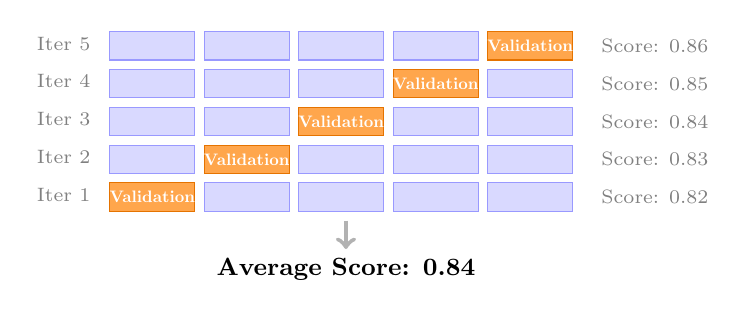
\begin{tikzpicture}[scale=0.6]
        \foreach \y in {0,1,2,3,4} {
             \node[left, font=\scriptsize, gray] at (-0.2, \y*0.8 + 0.35) {Iter \the\numexpr\y+1};
             \foreach \x in {0,1,2,3,4} {
                \ifnum \x=\y
                    % Test Fold
                    \draw[fill=orange!70, draw=orange!90!black] (\x*2, \y*0.8) rectangle (\x*2+1.8, \y*0.8+0.6);
                    \node[scale=0.6, font=\bfseries, white] at (\x*2+0.9, \y*0.8+0.3) {Validation};
                \else
                    % Train Fold
                    \draw[fill=blue!15, draw=blue!40] (\x*2, \y*0.8) rectangle (\x*2+1.8, \y*0.8+0.6);
                \fi
             }
             \node[right, font=\scriptsize, gray] at (10.2, \y*0.8+0.3) {Score: 0.\the\numexpr82+\y};
        }
        
        % Average Visual
        \draw[->, ultra thick, gray!60] (5, -0.2) -- (5, -0.8);
        \node[below, black, align=center, font=\small\bfseries] at (5, -0.8) {Average Score: 0.84};
    \end{tikzpicture}
\end{frame}

% --- SLIDE 3: K-FOLD SOLUTION ---
\begin{frame}{The Solution: K-Fold Cross Validation}

    \begin{tcolorbox}[colback=darkblue!5, colframe=darkblue!90, title=Why K-Fold Works]
        Every data point serves as a test sample exactly once. We evaluate on \textbf{100\%} of the data instead of just 20\%, removing the luck factor.
    \end{tcolorbox}

    \vspace{1.5em}
    \centering
    
    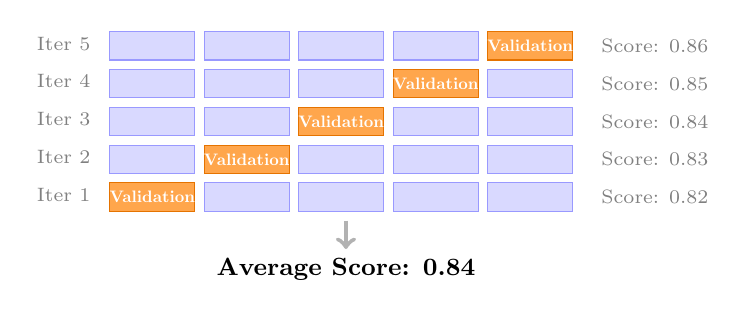
\begin{tikzpicture}[scale=0.6]
        \foreach \y in {0,1,2,3,4} {
             \node[left, font=\scriptsize, gray] at (-0.2, \y*0.8 + 0.35) {Iter \the\numexpr\y+1};
             \foreach \x in {0,1,2,3,4} {
                \ifnum \x=\y
                    % Test Fold
                    \draw[fill=orange!70, draw=orange!90!black] (\x*2, \y*0.8) rectangle (\x*2+1.8, \y*0.8+0.6);
                    \node[scale=0.6, font=\bfseries, white] at (\x*2+0.9, \y*0.8+0.3) {Validation};
                \else
                    % Train Fold
                    \draw[fill=blue!15, draw=blue!40] (\x*2, \y*0.8) rectangle (\x*2+1.8, \y*0.8+0.6);
                \fi
             }
             \node[right, font=\scriptsize, gray] at (10.2, \y*0.8+0.3) {Score: 0.\the\numexpr82+\y};
        }
        
        % Average Visual
        \draw[->, ultra thick, gray!60] (5, -0.2) -- (5, -0.8);
        \node[below, black, align=center, font=\small\bfseries] at (5, -0.8) {Average Score: 0.84};
    \end{tikzpicture}
    
\end{frame}

% --- SLIDE 3: K-FOLD SOLUTION ---
\begin{frame}{The Solution: K-Fold Cross Validation}

    \begin{tcolorbox}[colback=darkblue!5, colframe=darkblue!90, title=Why K-Fold Works]
        Every data point serves as a test sample exactly once. We evaluate on \textbf{100\%} of the data instead of just 20\%, removing the luck factor.
    \end{tcolorbox}

    \vspace{1.5em}
    \centering
    
    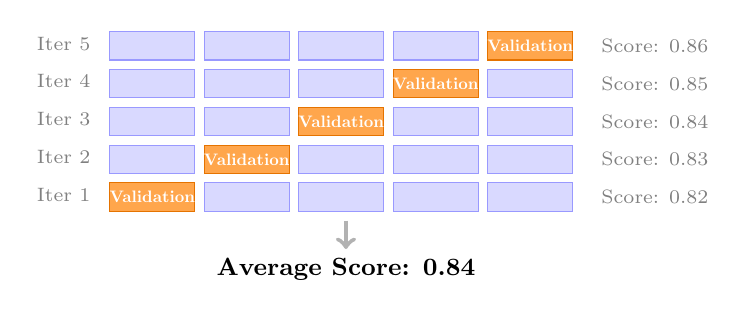
\begin{tikzpicture}[scale=0.6]
        \foreach \y in {0,1,2,3,4} {
             \node[left, font=\scriptsize, gray] at (-0.2, \y*0.8 + 0.35) {Iter \the\numexpr\y+1};
             \foreach \x in {0,1,2,3,4} {
                \ifnum \x=\y
                    % Test Fold
                    \draw[fill=orange!70, draw=orange!90!black] (\x*2, \y*0.8) rectangle (\x*2+1.8, \y*0.8+0.6);
                    \node[scale=0.6, font=\bfseries, white] at (\x*2+0.9, \y*0.8+0.3) {Validation};
                \else
                    % Train Fold
                    \draw[fill=blue!15, draw=blue!40] (\x*2, \y*0.8) rectangle (\x*2+1.8, \y*0.8+0.6);
                \fi
             }
             \node[right, font=\scriptsize, gray] at (10.2, \y*0.8+0.3) {Score: 0.\the\numexpr82+\y};
        }
        
        % Average Visual
        \draw[->, ultra thick, gray!60] (5, -0.2) -- (5, -0.8);
        \node[below, black, align=center, font=\small\bfseries] at (5, -0.8) {Average Score: 0.84};
    \end{tikzpicture}

    \begin{itemize}
                \item Only one problem left...
            \end{itemize}

    
    
\end{frame}



% --- SLIDE 1: IMBALANCE MOTIVATION (The Accuracy Paradox) ---
\begin{frame}{The Hidden Trap: Imbalanced Data}

    \begin{columns}[c]
        % --- Left Column: The Concept ---
        \begin{column}{0.45\textwidth}
            \textbf{What is Imbalance?}
            \begin{itemize}
                \item When one class dominates the target (e.g., 99\% Healthy, 1\% Sick).
            \end{itemize}
            
            \vspace{1em}
            \begin{alertblock}{The Accuracy Paradox}
                If you have 99 blue dots and 1 red dot, a model that \textbf{always guesses Blue} has 99\% Accuracy!
                \vspace{0.5em}
                
                But it failed to find the one thing we cared about!
            \end{alertblock}
        \end{column}
        
        % --- Right Column: The Visual ---
        \begin{column}{0.55\textwidth}
            \centering
            
            % 1. The Full Dataset
            \textbf{1. Target Distribution} \\(95\% Blue, 5\% Red)
            \vspace{0.2em}
            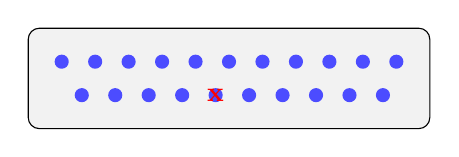
\begin{tikzpicture}[scale=0.85]
                \draw[fill=gray!10, rounded corners] (0,0) rectangle (6,1.5);
                % Lots of Blue
                \foreach \x in {0.5,1.0,1.5,2.0,2.5,3.0,3.5,4.0,4.5,5.0,5.5} 
                    \fill[blue!70] (\x, 1.0) circle (3pt);
                \foreach \x in {0.8,1.3,1.8,2.3,2.8,3.3,3.8,4.3,4.8,5.3} 
                    \fill[blue!70] (\x, 0.5) circle (3pt);
                
                % One tiny Red dot (The Needle)
                \node[red, font=\bfseries] at (2.8, 0.5) {x};
            \end{tikzpicture}
            
            \vspace{0.8em}
            
            % 2. Random Split Failure
            \textbf{2. Random Split}
            \vspace{0.2em}
            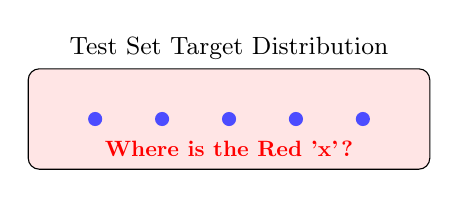
\begin{tikzpicture}[scale=0.85]
                % Test Set Box
                \draw[fill=red!10, rounded corners] (0,0) rectangle (6,1.5);
                \node[above, font=\small] at (3,1.5) {Test Set Target Distribution};
                
                % It picked only Blue
                \foreach \x in {1.0, 2.0, 3.0, 4.0, 5.0} 
                    \fill[blue!70] (\x, 0.75) circle (3pt);
                
                % Warning Label
                \node[red, font=\bfseries, scale=0.8] at (3, 0.3) {Where is the Red 'x'?};
            \end{tikzpicture}
  
        \end{column}
    \end{columns}
\end{frame}

% --- SLIDE 2: STRATIFICATION (The Solution) ---
\begin{frame}{The Fix: Stratified Splitting}

    \begin{block}{Definition}
        \textbf{Stratification} forces the Train and Test splits to preserve the \textbf{same class ratios} as the original dataset.
    \end{block}

    \vspace{1em}
    \centering
    
    \begin{columns}[c]
        % Visualizing the Force Split
        \begin{column}{0.6\textwidth}
            \centering
            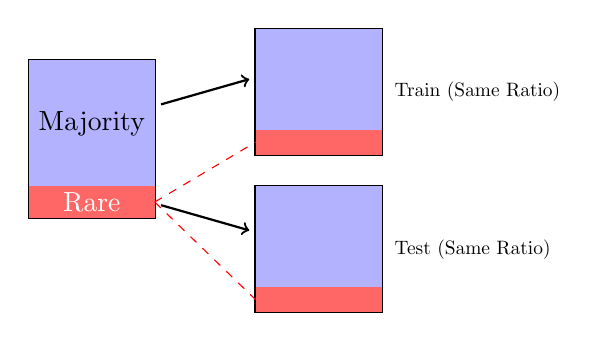
\begin{tikzpicture}[scale=0.8]
                % Full Data
                \draw[thick] (0,0) rectangle (2,2.5);
                \fill[blue!30] (0,0.5) rectangle (2,2.5); \node at (1,1.5) {Majority};
                \fill[red!60] (0,0) rectangle (2,0.5); \node[white] at (1,0.25) {Rare};
                
                % Arrows
                \draw[->, thick] (2.1, 1.8) -- (3.5, 2.2);
                \draw[->, thick] (2.1, 0.2) -- (3.5, -0.2);
                
                % Train
                \draw[thick, fill=blue!10] (3.6, 1.0) rectangle (5.6, 3.0);
                \fill[blue!30] (3.6, 1.4) rectangle (5.6, 3.0);
                \fill[red!60] (3.6, 1.0) rectangle (5.6, 1.4);
                \node[right, scale=0.7] at (5.7, 2.0) {Train (Same Ratio)};
                
                % Test
                \draw[thick, fill=blue!10] (3.6, -1.5) rectangle (5.6, 0.5);
                \fill[blue!30] (3.6, -1.1) rectangle (5.6, 0.5);
                \fill[red!60] (3.6, -1.5) rectangle (5.6, -1.1);
                \node[right, scale=0.7] at (5.7, -0.5) {Test (Same Ratio)};
                
                % Connection Lines indicating forced movement
                \draw[dashed, red] (2, 0.25) -- (3.6, 1.2);
                \draw[dashed, red] (2, 0.25) -- (3.6, -1.3);
            \end{tikzpicture}
        \end{column}
        
        % Text Explanation
        \begin{column}{0.4\textwidth}
            \textbf{Why it works:}
            \begin{itemize}
                \item It guarantees the Test set includes the "Red 'x'".
                \item It allows us to calculate metrics like Recall and F1-Score properly.
            \end{itemize}
            
            \vspace{1em}
            \begin{tcolorbox}[colback=green!5, colframe=green!40]
                \centering \small
                \textbf{Tip:}\\
                Use \textbf{Stratified K-Fold} for the best of both worlds!
            \end{tcolorbox}
        \end{column}
    \end{columns}
    
\end{frame}


\subsection{Performance Measurements (Metrics)}

\begin{frame}{Addressing Overfitting}
    \centering
    \large \textit{Since we cannot trust the training error, we need a systematic approach to validate our models.}
    
    \vspace{0.8cm}
    
    \begin{columns}[T]
        \begin{column}{0.3\textwidth}
            \begin{block}{\centering1. Detect:}
                \centering
                \textbf{Splitting Data}\\
                (Holdout, K-Fold)
            \end{block}
        \end{column}
        \begin{column}{0.3\textwidth}
            \begin{block}{\centering2. Measure:}
                \centering
                \textbf{Metrics}\\
                (Accuracy, MSE, F1, AUC)
            \end{block}
        \end{column}
        \begin{column}{0.3\textwidth}
            \begin{block}{\centering3. Mitigate:}
                \centering
                \textbf{Strategies}\\
                (Regularization, More Data, Better Features)
            \end{block}
        \end{column}
    \end{columns}
    
    \vspace{0.5cm}
    \centering
    \small $\rightarrow$ \textit{Step 1: How to simulate "unseen data" using Splits.} \\
    \small $\rightarrow$ \textit{Step 2: How to measure performance using Metrics.}
\end{frame}

% --- PART 2: MEASUREMENT ---


% --- SLIDE 1: INTRO (What & Why) ---
